\section{Introduction}
  \label{sec:intro}
\begin{figure}
\centering
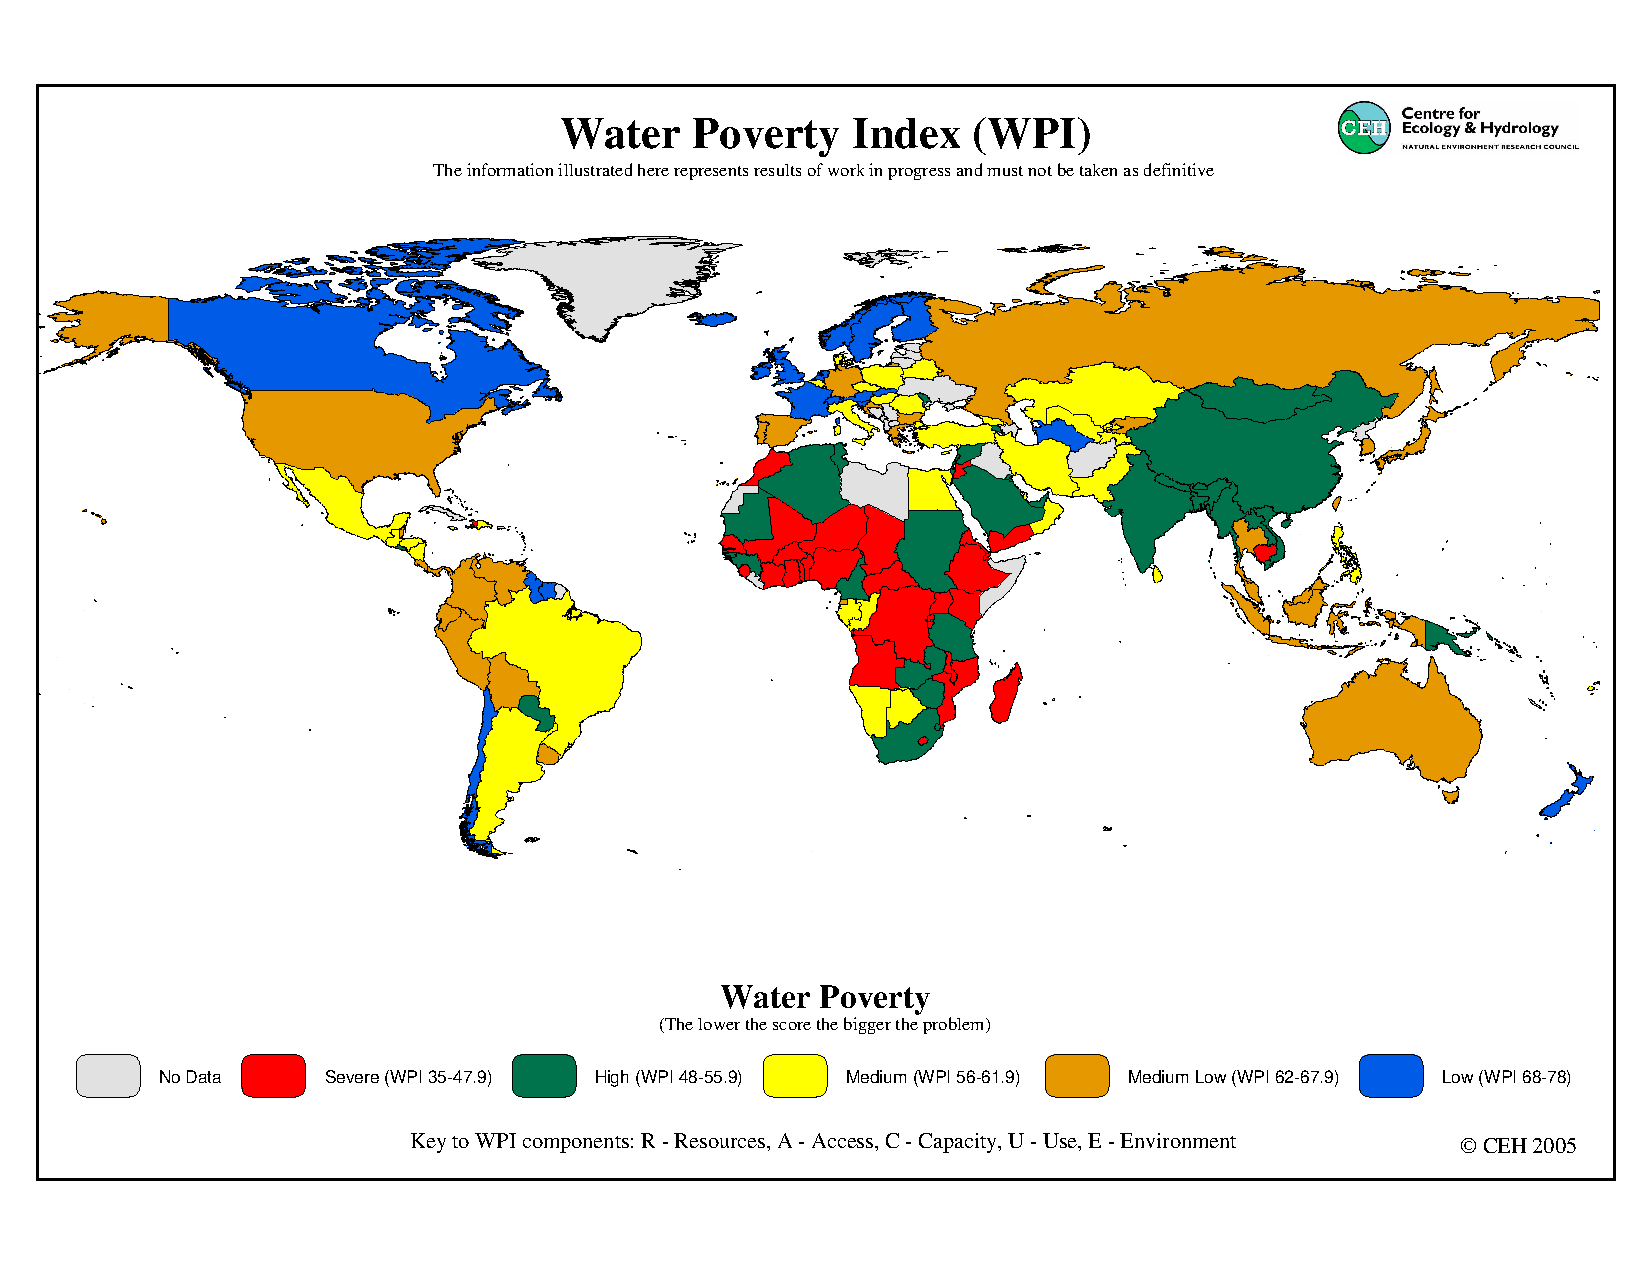
\includegraphics[width=90mm]{.//figures/WPIworldmap_2.pdf}
\caption{2005 Water Poverty Index (WPI)}
\vskip -6pt
\end{figure}
%%%%%Narrative

One day, Bob came home and checked his water bill. He was surprised with the extraordinary fee that he never paid before. He was wondering if there was significant wastage of water in his house. He wasn't sure about the fee and decided to call the water utility company one day to ask about it. 
Then he turned on a radio and was taking a shower. The radio was about the water poverty index over the world and was telling that many countries lack significant amount of water.

%%%%
Immediate actions to conserve natural resources are needed to be taken by all the people in the world, and ??? claimed that everyone needs to be a detective regarding their resource footprint. The available information regarding natural resources lacks spatial granularity as installation cost for the monitoring system in that level of granularity is significantly high and is not viable. 
[McMakin] [Stern] showed in their studies that the spatio-temporally finer grained information regarding natural resource usage pattern helps people pinpoint their resource usage pattern thus help improve their efficiency. 
%%%%%







Many countries lack significant amount of water. Water conservation has long been of great interest as its production cost become significant while demands grow rapidly. Figure 1 shows water poverty index in 2005 that illustrate demands for water resource of most of countries. 

Water flow monitoring is of great interest because it provides indices of water usage. Water flow rate measurement can be seen in several categories; 1) open channel water flow estimation, 2) open pipe water flow rate estimation, and 3) closed pipe water flow rate measurement. 1) and 2) are used especially for very large irrigation system as most of water channels are open. Distributed irrigation control is one of great examples of wireless sensors and actuators network that leverages spatially distributed water flow rate of open channels in real-time to optimize water usage for irrigation systems[].

Closed pipe water rate measurement is useful for many industrial industries for their production processes and most of houses and buildings for billing purpose. It can be divided into two categories; 1) intrusive direct water flow measurement and 2) nonintrusive water flow estimation. One very common example of intrusive direct water flow measurement technique is the main water flow meter that is widely deployed in most of houses for billing purpose. Many different types of intrusive water flow meter are available for industrial purpose[][]. This class of techniques always comes with high installation cost as it requires plumbing unless it is initial pipe construction. 

Nonintrusive water flow rate estimation technique that many researchers have focused on [][] has a merit as it doesn�t require us to install a sensor in a pipe. Ultrasonic water flow meter uses ultrasonic transmitter and receiver pair to measure water flow induced doppler shift. Commercially available products guarantee its precision up to ??. But its price is about \$1000 or more than that[Dynasonics]
Recently, vibration based [evan] water flow rate technique was developed. However, it is calibration intensive thus well trained technician is necessary to provide at least good quality of information. 

The traditional way of measuring the resource consumption is very coarse-grained; typically at household level and monthly basis. If we consider it as a feedback information for users to conserve natural resources, it gives only a partial and coarse awareness of resource consumption. However, measurement of water at an individual faucet level would help us pinpoint places and/or trends where they tend to consume more water, and thus improve resource efficiency by adjusting them according to spatially finer grained information. For example, Stern [1] and McMakin [3] showed that people are willing to conserve natural resources as their desire to do the right thing, and to save  cost. 

Environmental concerns also motivate [3] individuals to have finer grained information to be more aware of where they spend the most resources [18]. For these reasons, demand for such feedback information emerges. We believe that profiling at a finer granularity aids in pinpointing consumption patterns to improve resource efficiency. 

Although there were some attempts to monitor spatially finer grained water flow rate for irrigation systems and industrial purposes, there�s no application that profiles individual pipe level water flow rate for houses and buildings in less intrusive ways due to its cost and maintenance issues. 
We propose NAWMS, a scalable water monitoring system that is capable of estimating individual pipe level water consumption profile using sensor network technology while guaranteeing its minimum error of total water consumption estimate. The goal of NAWMS is to give people the possibility to monitor their own spatially distributed water consumption, i. e. water consumption of dish-washer, shower booth, bathroom sink, kitchen sink, sprinkler, etc.  To make it easily installable and deployable by non-experts, we took special care in NAWNS�s design to use COTS components that are non-intrusive (don�t have to cut pipes) and that are installable by everyone. 

The rest of the paper is structured as follows. In Section 2,  we describe related work. Section 3 details problem description and formulation. In section 4 we give detailed information on the NAWMS system architecture and describe its challenges. In section 5, we evaluate our prototype system against the ground truth and its performance. Then we discuss lessons from the deployment in Section 5 then conclude in Section 6.